\section{Experimental Evaluation}
\begin{figure*}[ht]

    \begin{subfigure}[b]{0.25\linewidth}
        \centering
        %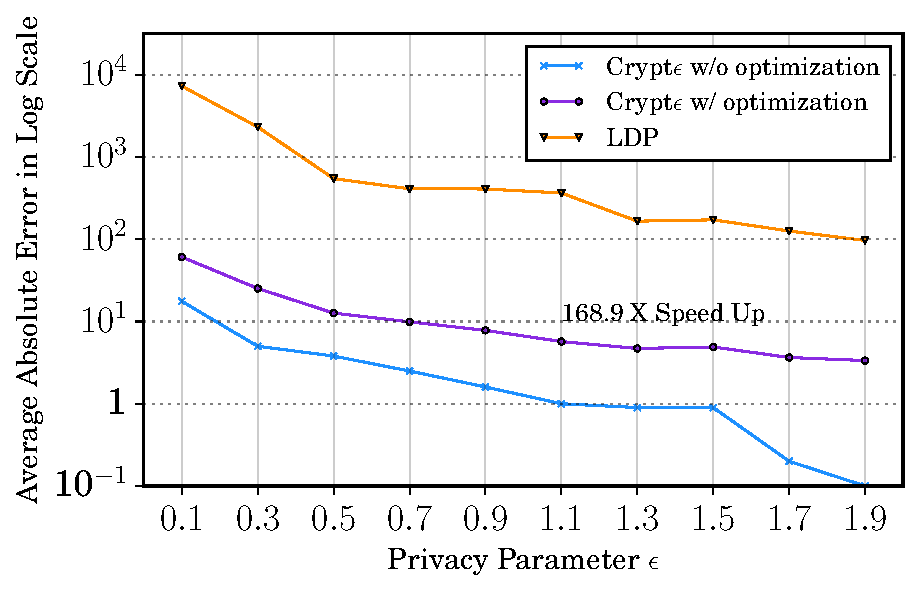
\includegraphics[width=5cm,height=3.1cm]{t1.pdf}
         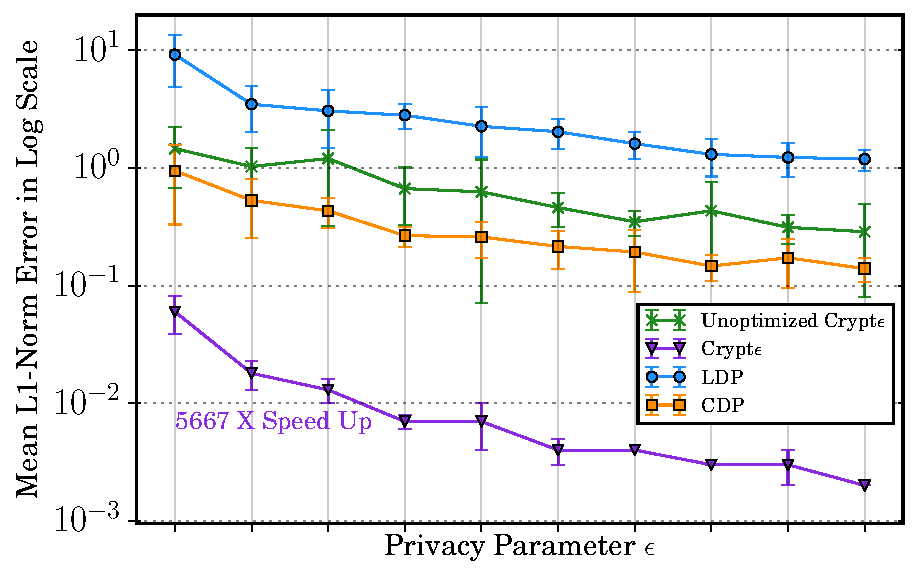
\includegraphics[width=1\linewidth]{t8_final.pdf}
        \caption{ Program 1}
        \label{fig:P1}
    \end{subfigure}%%
    \begin{subfigure}[b]{0.25\linewidth}
    \centering 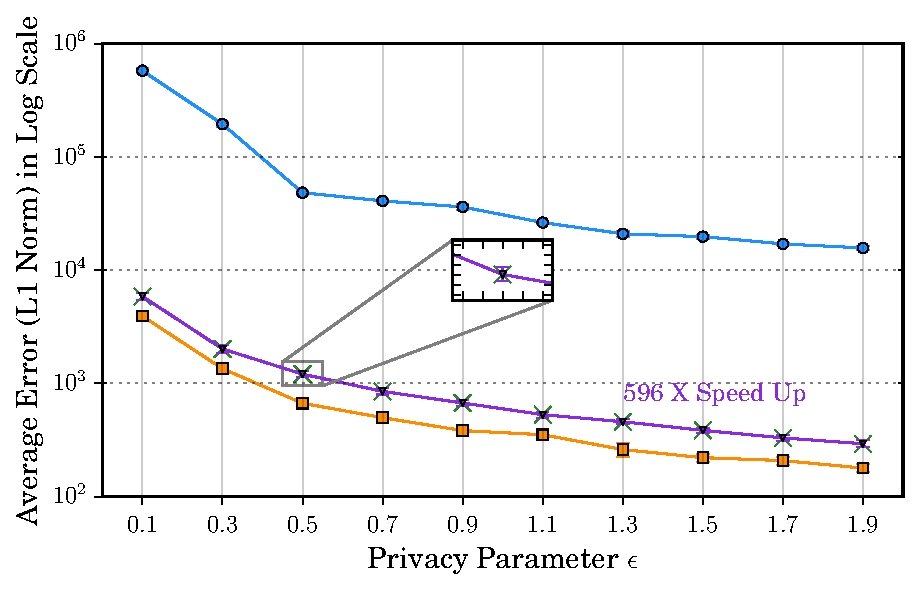
\includegraphics[width=1\linewidth]{3_final.pdf}
        \caption{Program 3}
        \label{fig:P3}\end{subfigure}%%
    \begin{subfigure}[b]{0.25\linewidth}
    \centering    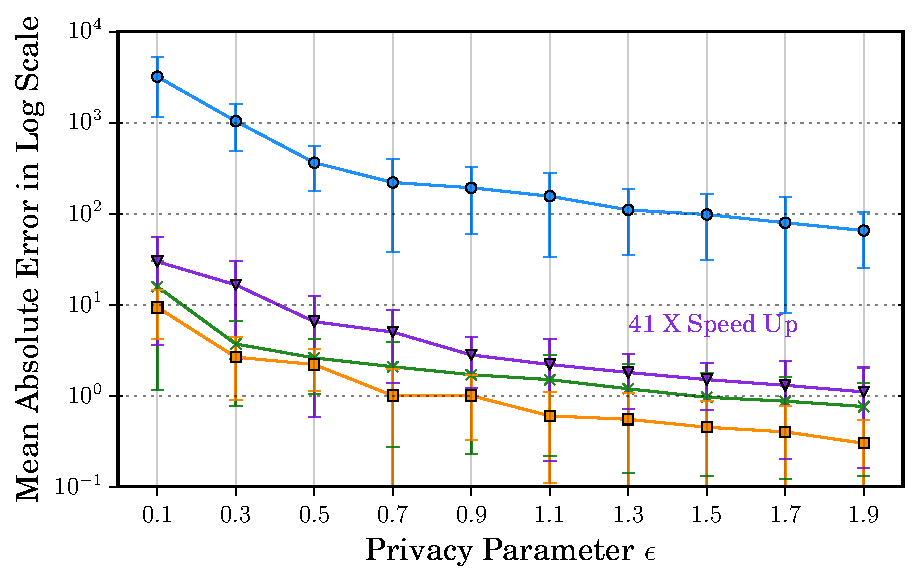
\includegraphics[width=1\linewidth]{5_final.pdf}
        \caption{Program 5}
        \label{fig:P5}\end{subfigure}%%
      \begin{subfigure}[b]{0.25\linewidth}
    \centering    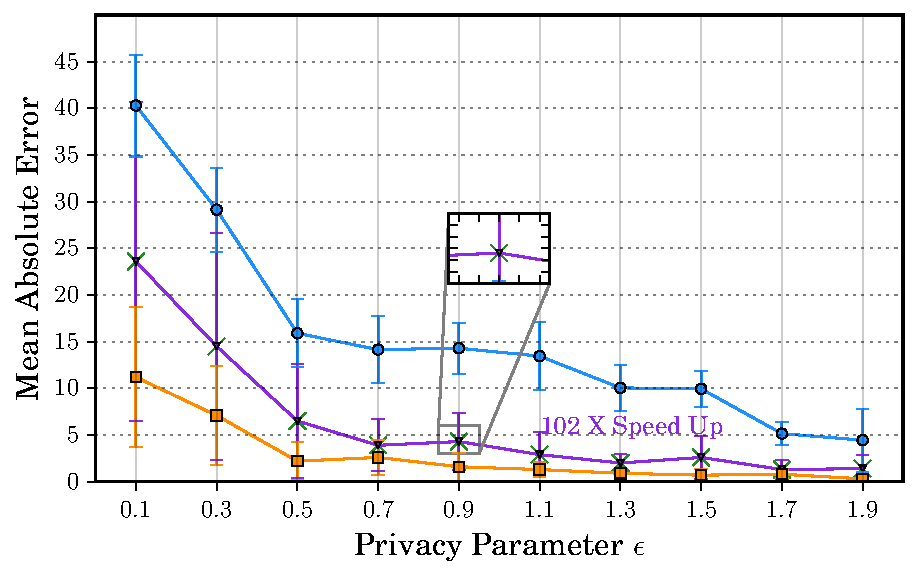
\includegraphics[width=1\linewidth]{7_final.pdf}
        \caption{Program 7}
        \label{fig:P7}
    \end{subfigure}
   \caption{Accuracy Analysis of Crypt$\epsilon$ Programs}
   \label{accuracy}
\end{figure*}
In this section we describe our evaluation of Crypt$\epsilon$ along two dimensions, accuracy and  performance of Crypt$\epsilon$ programs. Specifically we address the following questions : \squishlist \item \textbf{Q1:} Does Crypt$\epsilon$ programs have significantly lower error than that for the corresponding state-of-the-art \textsf{LDP} implementations?\item \textbf{Q2:} Does the proposed optimizations provide substantial performance improvement over unoptimized Crypt$\epsilon$? \item \textbf{Q3:} Is the execution time for Crypt$\epsilon$ programs practical and do they scale well? \squishend
%For the rest of the section, we consider the optimized implementation to be the default implementation for \system.\\
\textbf{Evaluation Highlights:}
\squishlist \item \system can achieve upto 2 orders of smaller error than the corresponding
\textsf{LDP} implementation on a data of significant size ($\sim 30,00$) (Figure \ref{accuracy}).
\item The optimization techniques in \system can improve the performance
of unoptimized \system by up to $6514\times$ (Table \ref{perf}).
\item The performance cost of a large class of \system programs is
less than 5 minutes for a data set of size $\sim 30,000$  and it scales linearly with the size of the data set (Figure \ref{scale}). The \textsf{AS} performs majority of the work for most program executions (Table \ref{perf}).
\squishend
\subsection{Methodology} 
\textbf{Programs:}
To answer the aforementioned questions we ran the experiments on the Crypt$\epsilon$ programs previously outlined in Table 3. Due to space limitations we present the results of only four of them in the main paper namely P1,P3,P5 and P7. The rationale behind choosing these four is that they cover all three classes of programs (section 5.3) and showcase the advantages for all of the four proposed optimizations. %Each program is compared with the corresponding state-of-the-art \textsf{LDP} implementation \cite{LDP1}.
Additional experimental results for programs P1,P3 and P5 from Table \ref{tab:programexamples} are presented in Appendix.% We rename the examples 5.1,5.2,5.3,5.4,5.6 and 5.7 as P1,P1,P5,. The reason behind this grouping is to arrange the programs in their increasing order of complexity.  %\begin{itemize}\item \textbf{Program 1} - Count the number of records having age in range $[50,60]$ \\\textbf{\textsf{LDP} Competitor} - Frequency oracle of \cite{LDP1} constructed over attribute $Age$. \item \textbf{Program 2} - Report the top 5 most frequent age values. \\\textbf{\textsf{LDP} Competitor} - Frequency oracle of \cite{LDP1} constructed over attribute $Age$.  \item \textbf{Program 3 }- Report the marginal on attributes $Age$ and $Gender$. \\\textbf{\textsf{LDP} Competitor }- Frequency oracle of \cite{LDP1} constructed over attribute $Age \times Gender$. \item \textbf{Program 4 }- Report the marginal on attributes $Age$ and $Gender$ with $NativeCountry=Mexico$\\\textbf{\textsf{LDP} Competitor }- Frequency oracle of \cite{LDP1} constructed over attribute $Age\times Gender \times NativeCountry$. \item \textbf{Program 5 }- Count the number of natively Mexican male employees of age 30.\\\textbf{\textsf{LDP} Competitor }- Frequency oracle of \cite{LDP1} constructed over attribute $Age\times Gender \times NativeCountry$. \item \textbf{Program 6 }- Count the number of distinct age values for male employees. \\\textbf{\textsf{LDP} Competitor }-Frequency oracle of \cite{LDP1} constructed over attribute $Age\times Gender$.% and reports the number of non-zero counts after suitable adjustment for thresholding. 
%\item \textbf{Program 7 }- Count the number of age values with at least 10 records. \\\textbf{\textsf{LDP} Competitor }- Frequency oracle of \cite{LDP1} constructed over attribute $Age$. \end{itemize}
\\\textbf{Data set:}
We ran our experiments on the Adult data set from the University of California, Irvine CI repository \cite{UCI}  which has been extracted from the 1994 census data. The data set is of size $32,651$.
\\\textbf{Metrics:}
\\\textit{Accuracy:} For accuracy the following metrics are used
\squishlist \item Programs with scalar outputs, i.e.,  P5 and P7 use absolute error $ =|c-\hat{c}|$ where $c$ is the true count and $\hat{c}$ is the noisy output.\item Programs with vector outputs, i.e., P1 and P3 uses the L1 error metric given  by $Error=\sum_{i}|V[i]-\hat{V}[i]|, i \in [|V|]$.\\
For each of the programs, we report the mean error values over 10 repetitions.\squishend
\textit{Performance}: For measuring performance we report the mean total execution time in seconds for each program, over 10 repetitions. \textbf{Configuration:} We implemented \system in Python with the garbled circuit implemented via the EMP
toolkit \cite{EMP}. The prototype also includes all four 
optimization described in section 6.
For Adult data set, \system constructs a DP index optimization over
the attribute $NativeCountry$ that benefits programs like P4 and P5. Our experiments assign
20\% of the total program privacy parameter towards constructing the index
and the rest is used for the remaining program execution. \system also constructs a
DP range tree over the attribute $Age$ with the full privacy parameter. This helps programs like P1,P2 and P3. This is our default implementation for \system. %We refer to the implementation without the optimization as  unoptimized \system. 
% We evaluated our prototype on 3 servers each with configuration 32GB RAM, 1TB SSD, and
%2.6GHz 6-core 8th-generation Intel Core i7 processor and  macOS.

%uses the error measure given by the fraction of age values returned in the top 5 that have value less than $ct_5-\alpha$  where  $ct_5$ is the count of the $5^{th}$ largest value and $\alpha=\frac{1}{\epsilon}\log\frac{1}{\delta}$ is a slack parameter. The slack parameter is required because with probability $1-\delta$ no differentially private algorithm can distinguish between any two counts that differ by less than $\alpha$. We use $\delta=0.05$ for our experiment. \item Programs 3, 4 and 5 \end{itemize}


\subsection{Experimental Results}\label{exp:results}
\subsection*{Accuracy}
In this section we evaluate \textbf{Q1} by performing a comparative analysis between the empirical accuracy of the aforementioned four \system programs (both optimized and unoptimized) and that of the corresponding state-of-the-art \textsf{LDP} \cite{LDP1} and \textsf{CDP} \cite{Dork} implementations  with varying privacy parameter $\epsilon \in \{0.1,...,0.9\}$. %All the experiments are evaluated on the full dataset and we report our results for 
The first observation with respect to accuracy is that the mean error for a single frequency count for Crypt$\epsilon$ is at least 2 orders less than that of the corresponding \textsf{LDP} implementation.   For e.g., Figure \ref{fig:P1} shows that for P1 (c.d.f on $Age$), the mean error for \system for $\epsilon=0.1$ is given by $0.060$ while the corresponding \textsf{LDP} implementation has an error of $9.2$. Similarly for P3 (Figure \ref{fig:P3}),  $\epsilon=0.1$ results in a mean error of $5862.4$ as compared to an error of $576478.2$ for the corresponding \textsf{LDP} implementation. P5 (Figure \ref{fig:P5}) gives a mean error of only $15.8$ for $\epsilon=0.1$. In contrast, the corresponding \textsf{LDP} implementation has an error of $3199.96$.   The accuracy
improvement on P7 (Figure \ref{fig:P7}) by \system is less significant as compared to the other programs. It is so because, P7 outputs the number of age values ([1-100]) having at least
100 records. At $\epsilon=0.1$, at least 40 age values out of 100 are
reported incorrectly on whether their counts pass the threshold. \system reduces the error by half. 

For P1 (Figure \ref{fig:P1}), we observe that the error of \system is around an order less than that of the unoptimized implementation. For instance, the mean error for \system is $20\times$ lower than that of unoptimized \system for $\epsilon=0.1$.  The reason is that, P1 constructs the c.d.f over the attribute $Age$ (with domain size 100) by first executing 100 range queries. %, where the $i$-th query outputs the noisy count for age values in $[1,i], i \in [100]$. This is followed by an isotonic regression post-processing to get a proper c.d.f.
Thus, if the total privacy budget for the program is $\epsilon$, then for unoptimized \system, each query gets a privacy parameter of just $\frac{\epsilon}{100}$. In contrast, the DP range tree is constructed with the full budget $\epsilon$ and sensitivity $\lceil\log 100\rceil$ thereby resulting in lesser error. For P5 (Figure \ref{fig:P5}) however, the unoptimized implementation has slightly better accuracy (around $2\times$) than \system. It is because of two reasons; firstly the noisy index on $NativeCountry$ might miss some of the rows satisfying the filter condition ($NativeCountry$=Mexico). Secondly, since only 0.8\% of the total privacy parameter is earmarked for the \textsf{Laplace} primitive in the optimized program execution, this results in a higher error as compared to that of unoptimized \system. However, this a small  cost to pay for achieving a performance gain of $41\times$. The optimizations for P3 (Figure \ref{fig:P3}) and P7 (Figure \ref{fig:P7}) work completely on the encrypted data and do not expend the privacy budget. Hence they do not hurt the program accuracy in any way.
 
 Another observation from Figure \ref{accuracy} is that the error of \system is around $2\times$ higher than that of the corresponding \textsf{CDP} implementation. This conforms with our expectation as we add two instances of Laplace noise in \system. For instance, \system's error for programs 4 (Figure \ref{fig:P3}), 6 (Figure \ref{fig:P5}) and 8 (Figure \ref{fig:P7})  is respectively $1.49\times$, $1.69 \times$ and $2.1\times$ higher  than that of the corresponding \textsf{CDP} implementation for $\epsilon=0.1$.  For P1 however \system has at least $15\times$ lower error than that of the \textsf{CDP} implementation due to the DP range tree optimization as explained in the preceding paragraph.
 

\subsection*{Performance Gain Due to Optimizations}
In this section we evaluate \textbf{Q2} by analysing how much speed-up is brought about by the proposed optimizations in the total program execution. The results are reported in Table \ref{perf}.
 \eat{\begin{table}[ht]
\caption{Execution Time Analysis for Crypt$\epsilon$ Programs}
\small
\centering
\begin{tabular}{c  c c c c c}
\toprule
Program &  \multicolumn{3}{c}{Base} & \multicolumn{2}{c}{Optimized} \\ 
 & AS &  CSP & Total & Total & Speed up  \\ &(s)&(s)&(s)&(s)&$\times$\\ % inserts table %heading
\midrule
1 & 0.49& 0.0027& 0.4927 & 0.0029 & 168.9 \\
2 &  6.12 & 0.3  &6.42 & 0.89 & 7.2\\ %197 the communication rounds
3&  3859.52 & 3661.29 & 7520.81&N/A&N/A \\4  &7765.16&3624.05&11389.21& 910.96 & 12.5 \\5&18.56&16.7&35.26&3.49 & 10.1 \\6&1910.01&571.11&2481.12&429.92 & 5.77\\7&6.35 & 1393.89 & 1400.24 &  N/A & N/A \\ [1ex]
\bottomrule
\end{tabular}
\label{c}
\end{table}}
\begin{table}
\caption{Execution Time Analysis for Crypt$\epsilon$ Programs}
\centering
\scalebox{0.78}{
\begin{tabular}{|c c|c|c|c|c|}
\hline
\multicolumn{2}{|c}{\textbf{Time in (s)}}   & \multicolumn{4}{|c|}{\textbf{Program}}\\
\cline{3-6}&&\textbf{1} & \bf{3} & \bf{5} &\bf{7}  \\ 
\hline \hline
\multirow{3}{*}{\textbf{Unoptimized \system}}& \multicolumn{1}{|c|}{\textsf{AS}} & 1756.71 &  101840.83 & 650.78&290   \\
\cline{2-6}& \multicolumn{1}{|c|}{\textsf{CSP}} & 0.26 & 78131.27& 550.34  &30407.73\\\cline{2-6}
& \multicolumn{1}{|c|}{Total} & 1756.97 & 179972& 1201.12 &30697.73    \\\hline
%\multirow{4}{*}{\textbf{Optimized}}& \multicolumn{1}{|c|}{\textsf{AS}} & .0004 &16.21 &250.17  &\\ \cline{2-6}& \multicolumn{1}{|c|}{\textsf{CSP}} & .0027 &13.92 &0.54 &\\
\multirow{2}{*}{\textbf{\system}}& \multicolumn{1}{|c|}{Total} & 0.31 &     301.53 & 29.21& 299.5 \\
\cline{2-6}& \multicolumn{1}{|c|}{Speed Up $\times$} &5667.64 &596.86& 41.1 &    102.49
\\ [1ex]
\hline
\end{tabular}}
\label{perf}
\end{table}
\\
\textit{DP Range Tree}
 For P1 we see that the total time taken for execution for the unoptimized Crypt$\epsilon$ implementation is about half an hour. However, using the range tree optimization reduces the execution time by $5667\times$. The reason behind this huge speed-up is that the time required by the \textsf{AS} in the optimized implementation becomes almost negligible because it simply needs to do a memory fetch to read off the answer from the pre-computed range tree instead of computing it from the entire encrypted database. 
 \begin{figure}[ht]
   \begin{subfigure}[b]{0.45\linewidth}
    \centering 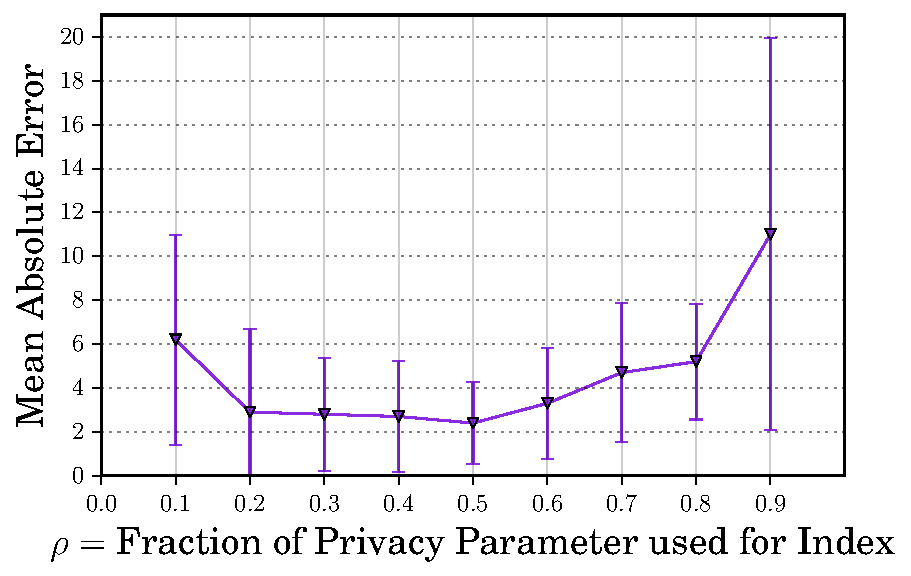
\includegraphics[width=1\linewidth]{index_error.pdf}
        \caption{}
        \label{fig:error}\end{subfigure}
        \begin{subfigure}[b]{0.45\linewidth}
        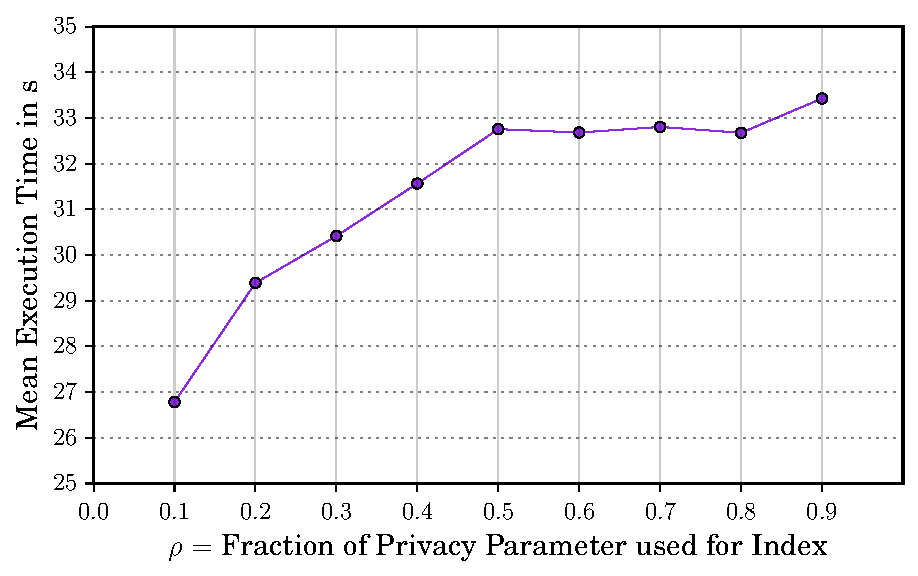
\includegraphics[width=1\linewidth]{index_time.pdf}
        \caption{}
        \label{fig:time}
        \end{subfigure}
        \caption{Program 5: Accuracy vs Performance Trade-off Analysis for DP Index Optimization }\label{index}
    \end{figure}
\\\textit{DP Index}- For P5, we observe that the base case implementation takes around $20$ minutes to run. However  a DP index over the attribute $NativeCountry$  reduces the execution time to about $30s$ giving us a $41\times $ speed-up. It is so because, only about 2\% of the data records satisfy $NativeCountry$=Mexico. Thus the index reduces the number of records to be considered for the program execution drastically thereby resulting in a huge performance boost. %The is because only the cost for the \textsf{Filter} primitive decreases, not all the primitives scale 10 drop is due to the 
Let $\rho$ represent the fraction of the privacy parameter used towards constructing the DP index. In Figure \ref{index} we study how the mean execution time and the error of the final result vary as a function of $\rho$ for P5 for a total privacy parameter of $\epsilon=1.1$.  From Figure \ref{fig:error} we observe that the mean error incurred drops sharply from $\rho=0.1$ to $\rho=0.2$, stabilises till $\rho=0.5$ and starts increasing again. This is so because, at $\rho=0.2$, the noisy index correctly identifies almost all the records satisfying the $\textsf{Filter}$ condition and hence does not contribute much to the total error. However as we keep increasing $\rho$, the amount of privacy budget left for the $\textsf{Laplace}$ primitive keeps decreasing which results in higher error. From Figure \ref{fig:time}, we observe that the execution time increases till $\rho=0.5$ and then stabilizes. The reason behind this is that, the total number of records returned after $\rho=0.5$ does not differ by much. Thus from the two figures we observe that for $\rho=0.2$ we get a high speed up ($40\times$) with relatively low error ($3$). Hence we choose $\rho=0.2$ for our experiments. A formal accuracy vs speed up trade-off analysis would be very helpful in this regard and is part of our future plan.
 \\\textit{Pre-computation}- For P3 the unoptimized execution time on the data set of $32561$ records is around 2 days. This is so because the $\textsf{CrossProduct}$ primitive used in the program needs to perform $200\cdot 32561$ $labMult$ operations which is very time consuming. Hence from Table \ref{perf} we see that, pre-computing the 2-D attribute over $Age$ and $Gender$ is a very useful optimization as now the execution reduces to just about 5 minutes giving us a $596.86\times$ speed up. \\ %The un-optimized implementation for  Program D takes . It is because of the \textsf{CrossProduct} Primitiev because ot needs to compute . Pre-computaion f thsi saves a lot of time and cuts down the executioj tiem by.
\textit{Off-line Processing}-
The costliest primitive for P7 is the \textsf{GroupByCount} primitive since the \textsf{CSP} has to generate $3256200$ ciphers of $0$ and $1$ for the encrypted one-hot-codings and the total execution time in unoptimized \system is about 8.5 hours. But by generating the ciphers off-line, the execution time can be reduced to just $5$ minutes giving us a speed up of $102.49\times$.
Another important observation from Table \ref{perf} is that the \textsf{AS} performs the major chunk of the work for most program executions. This conforms with our discussion in section 3.6.
 \begin{figure}[ht]
    
     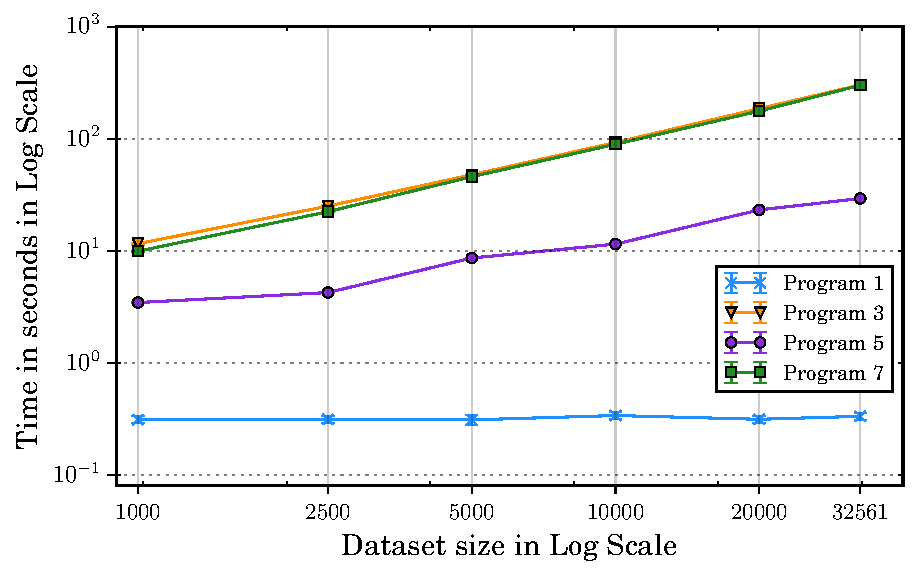
\includegraphics[width=0.5\linewidth]{scale_finals.pdf}
        \caption{Scalability of \system Programs }\label{scale}
    \end{figure}
 \subsection*{Scalability}
 In this section we evaluate \textbf{Q3} by observing the execution times of the aforementioned four \system programs and studying how well the programs scale (Figure \ref{scale}). All the reported execution times are for optimized implementations. For P1 we see that the the execution time remains unchanged for all the data set sizes. It is so because once the range tree is constructed, irrespective of the data set size, the program execution just involves reading the answer directly from the modes of the tree followed by a decryption by the \textsf{CSP}. The execution time for the optimized P3 is dominated by the cost of the $\oplus$ operation for the \textsf{GroupBy} primitive which scales linearly with the number of data records. Hence, as shown in Figure \ref{scale}, the execution time for P3 increases linearly with the data set size. For P5, the execution time basically depends on the \% of the records in the given data set that satisfy the condition $NativeCountry=Mexico$ (as this is roughly the number of records that will be retrieved from the noisy index). %From the figure, we observe that P5 too scales almost linearly with the dataset size. 
 For the optimized execution of P7  as well, the time is dominated by the $\oplus$ operation for the \textsf{GroupBy} primitive, thereby scaling linearly with the data set size.   %\subsection{Threats to Validity}- 
 %In Table 2 we report the execution time of  the aforementioned $7$ Crypt$\epsilon$ programs. For Program 1 we see that the total time taken for execution for the base case Crypt$\epsilon$ implementation is about 0.5 seconds; the cost is mainly dominated by the \textsf{AS} which has to make a pass through the entire encrypted database. The \textsf{CSP} on the other hand is just needed for decryption in the last step. Program 2 needs to compute the encrypted $Age$ histogram via $GroupBy*$ primitive which takes about $6$ seconds. The \textsf{CSP} time is also more than the previous case because of the garbled circuit in the $NoisyMax$ primitive. The total execution time for the base case implementation for Program 3 is roughly 2 hours.  The reason behind this comparatively higher timing as compared to that of the previous two programs is that the \textsf{CrossProduct} primitive requires  multiplication of the ciphers  which is costlier than the addition operator $\bigoplus$. For Program 4, we observe that the base case implementation takes around 3.1 hours to run. The timing is greater than that for Program 3 because, in this case the additional condition $NativeCountry=Mexico$ results in extra interactions with the \textsf{CSP}. Program 5 requires about $35$ seconds to execute in the base case while Program 6 runs for $41$ minutes. For Program 7 we see that the majority of the time is required by the \textsf{CSP} for generating the encrypted one-hot-codings for the $GroupBy$ primitive and takes $24$ minutes to execute.  An important observation throughout the experiments is that the time taken by the \textsf{AS} is significantly greater than that for the \textsf{CSP} for all the programs except for Program 7. This is a desirable trait for Crypt$\epsilon$ as discussed in section 3.6.








